\documentclass{article}
\usepackage[a4paper] {geometry}
\usepackage{xcolor}
\usepackage{listings}
\usepackage{graphicx}
\usepackage{colortbl}
\usepackage{color}
\definecolor{mygreen}{rgb}{0,0.6,0}
\definecolor{mygray}{rgb}{0.5,0.5,0.5}
\definecolor{mymauve}{rgb}{0.58,0,0.82}
\usepackage{float}
\usepackage[utf8]{inputenc}
\usepackage[italian]{babel}
\usepackage{gensymb}
\usepackage{textcomp}
\usepackage{bookmark}
\usepackage{titling}
\newcommand{\subtitle}[1]{%
	\posttitle{%
		\par\end{center}
	\begin{center}\large#1\end{center}
	\vskip0.5em}%
}
\usepackage{hyperref}
\hypersetup{
	pdfpagemode={UseOutlines},
	%bookmarksopen,
	pdfstartview={FitH},
	colorlinks,
	linkcolor={black},
	citecolor={red},
	urlcolor={blue}
}
\lstset{ 
	backgroundcolor=\color{white},   % choose the background color; you must add \usepackage{color} or \usepackage{xcolor}; should come as last argument
	basicstyle=\footnotesize,        % the size of the fonts that are used for the code
	breakatwhitespace=false,         % sets if automatic breaks should only happen at whitespace
	breaklines=true,                 % sets automatic line breaking
	captionpos=b,                    % sets the caption-position to bottom
	commentstyle=\color{mygreen},    % comment style
	deletekeywords={...},            % if you want to delete keywords from the given language
	escapeinside={\%*}{*)},          % if you want to add LaTeX within your code
	extendedchars=true,              % lets you use non-ASCII characters; for 8-bits encodings only, does not work with UTF-8
	firstnumber=1,                % start line enumeration with line 1
	frame=single,                          % adds a frame around the code
	keepspaces=true,                 % keeps spaces in text, useful for keeping indentation of code (possibly needs columns=flexible)
	keywordstyle=\color{blue},       % keyword style
	language=[x86masm]Assembler,                 % the language of the code
	morekeywords={*,...},            % if you want to add more keywords to the set
	numbers=left,                    % where to put the line-numbers; possible values are (none, left, right)
	numbersep=5pt,                   % how far the line-numbers are from the code
	numberstyle=\tiny\color{mygray}, % the style that is used for the line-numbers
	rulecolor=\color{black},         % if not set, the frame-color may be changed on line-breaks within not-black text (e.g. comments (green here))
	showspaces=false,                % show spaces everywhere adding particular underscores; it overrides 'showstringspaces'
	showstringspaces=false,          % underline spaces within strings only
	showtabs=false,                  % show tabs within strings adding particular underscores
	stepnumber=1,                    % the step between two line-numbers. If it's 1, each line will be numbered
	stringstyle=\color{mymauve},     % string literal style
	%tabsize=2,                      % sets default tabsize to 2 spaces
	title=\lstname                   % show the filename of files included with \lstinputlisting; also try caption instead of title
}

\date{}
\begin{document}
	\title{Relazione Sistemi Elettronici} 
	\subtitle{Descrizione della tesina: si realizzi un firmware che riceve dal computer (tramite porta seriale) una parola, come sequenza di codici ascii dei singoli caratteri. La parola è terminata da un punto ed è di lunghezza massima fissata a priori. Dopo aver ricevuto la parola, il programma deve reinviarla sulla porta seriale scritta al contrario.}
	\author{Matteo Orlandini\\Corso di Laurea Triennale in Ingegneria Elettronica\\Matricola 1079505}
	\maketitle
	\tableofcontents
	\newpage
	\section{Diagramma di flusso}
	\begin{figure}[H]
		\centering	
		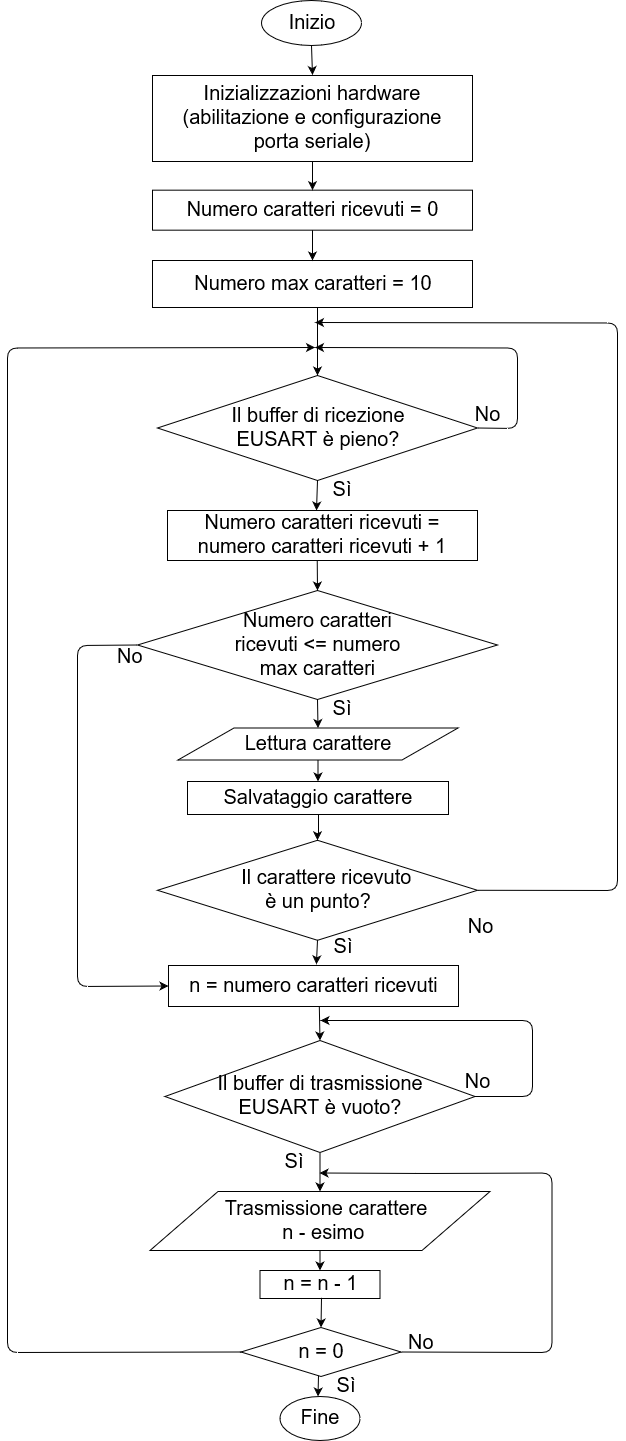
\includegraphics[width=0.57\textwidth]{Diagramma_di_flusso.png}
		%\caption{Diagramma di flusso}
		%\label{fig:label}
	\end{figure}
	\section{Codice}
	\subsection{Direttive}
	La direttiva list imposta il tipo di processore usato, cioè il PIC16F887. I "configuration bits" possono essere programmati per selezionare varie configurazioni del dispositvo. Questi bit sono mappati all'indirizzo 2007h della program memory. L'indirizzo 2007h è oltre lo spazio della program memory, appartiene infatti allo spazio special configuration memory compreso tra 2000h e 3FFFh, che può essere indirizzato solo durante la programmazione. I configuration bits sono impostati come riportato di seguito:
	\begin{itemize}
		\item \emph{CONFIG1}:
		\begin{itemize}
			\item \emph{\_INTRC\_OSC\_NOCLKOUT} $\rightarrow$ oscillatore interno: pin RA6/OSC2/CLKOUT e RA7/\\OSC1/CLKIN con funzioni di I/O
			
			\item \emph{\_WDT\_OFF} $\rightarrow$ Watch Dog Timer disabilitato, può essere abilitato dal bit \emph{SWDTEN} del registro \emph{WDTCON}.
			
			\item \emph{\_LVP\_OFF}$\rightarrow$ pin RB3 usato come I/O, High Voltage su MCLR usato per programmare.
		\end{itemize}
		\item \emph{CONFIG2}:
		\begin{itemize}
			\item 	\emph{\_BOR21V} $\rightarrow$ Brown-out Reset settato a 2.1 V.
		\end{itemize}
	\end{itemize}

	\begin{lstlisting}[frame=single] 
	#include "p16f887.inc"
	list p=16f887
	
	; configuration bits
	__CONFIG _CONFIG1, _INTRC_OSC_NOCLKOUT & _WDT_OFF & _LVP_OFF
	__CONFIG _CONFIG2, _BOR21V
	\end{lstlisting}
	
	
	\subsection{Inizializzazione variabili}
	\begin{enumerate}
		\item numeroChar contiene il numero attuale di caratteri ricevuti sulla seriale, viene inizializzato a zero.
		\item numeroMassimo contiene il numero massimo di caratteri che si possono inviare sulla seriale, viene inizializzato a 10.
		\item rxData contiene il dato ricevuto, letto da \emph{RCREG}.
		\item Inizializzo il puntatore File Select Register (FSR) al fine di puntare all'indirizzo 0x20, cioè al primo General Purpose Register disponibile.
	\end{enumerate}
	
	\begin{lstlisting}[frame=single]
;variabili in RAM (shared RAM)
			udata_shr
numeroChar		res		.1 
numeroMassimo		res		.1
rxData			res		.1

; reset vector
rst_vector		code	0x0000
			pagesel start
			goto start
		
	
	; programma principale
	code
start
	;inizializzo la variabile che conta i caratteri ricevuti
	movlw .0
	movwf numeroChar
	;inizializzo la variabile che contiene il numero massimo di 
	;caratteri che si possono ricevere
	movlw .10
	movwf numeroMassimo
	
	;inizializzo il puntatore al vettore che contiene i caratteri
	;per contenere l'indirizzo 0x20, cioe' il primo general purpose
	;file register
	movlw 0x20 
	movwf FSR
	
	pagesel initHw
	;initHw contiene le inizializzazioni hardware
	call initHw  
	\end{lstlisting}
	
	\subsection{Configurazioni hardware}
	\begin{enumerate}
		\item Gli interrupt sono tutti disabilitati, quindi il registro \emph{INTCON} ha tutti i bit a zero, perché il controllo sulla seriale viene fatto in polling. Questa scelta è dovuta al fatto che sarebbe possibile mandare il PIC in sleep e poi farlo svegliare tramite wake up da seriale, ma si perderebbe il primo byte ricevuto che servirebbe per l'uscita dallo stato di sleep del micro.	
		\item Disabilito tutti gli interrupt dalle periferiche resettando tutti i bit del registro PIE1.
		\item Dal registro \emph{OSCCON} imposto il clock a 8 MHz portando ad 1 i bit [6:4] e il bit 0 per usare l’oscillatore interno come clock di sistema.
		\item Nel registro \emph{OPTION\_REG} imposto il prescaler del timer 0 a 256 e l’interrupt sul fronte di discesa del pin INT. Il timer 0 viene impostato ma non è usato nel progetto.
		\item Tutte le porte sono settate in input perché non sono necessari degli output nel progetto.
		\item Il protocollo USART è configurato nei registri \emph{TXSTA}, \emph{RXSTA}, \emph{BAUDCTL} e \emph{SPBRG}.
		\begin {enumerate}
			\item In \emph{TXSTA}, i bit \emph{TXEN} e \emph{BRGH} sono ad 1 per indicare rispettivamente l'abilitazione della trasmissione e la trasmissione ad alta velocità. Il bit \emph{SYNC} è a zero perché viene selezionata la modalità asincrona.
			\item Nel registro \emph{RXSTA}, vengono abilitate la porta seriale e la ricezione continua settando i bit \emph{SPEN} e \emph{CREN}. 
			\item Si resettano tutti i bit di \emph{BAUDCTL}, tra cui anche \emph{BRG16}, impostando così il baud rate a 8 bit. 
			\item Con la configurazione citata, cioè \emph{SYNC} = 0, \emph{BRGH} = 1 e \emph{BRG16} = 0, la formula per calcolare il Baud Rate è la seguente: $$ Baud Rate = \frac{F_{osc}}{16\cdot(n+1)} $$ dove $F_{osc} = 8 MHz$ e n è il numero da inserire nel registro \emph{SPBRG}. Per avere un Baud Rate di 19200 bps, n deve essere pari a 25.
		\end{enumerate}
	\end{enumerate}
	\begin{lstlisting}[frame=single]
initHw
	;*********** inizio configurazioni hardware  *******************		
	
	;**********  inizio configurazione interrupt  ******************
	movlw B'00000000'
	banksel INTCON
	;INTCON:
	;bit 7 = 0 -> disabilitazione di tutti gli interrupt
	;bit 6 = 0 -> disabilitazione interrupt dalle periferiche
	;bit 5 = 0 -> disabilitazione interrupt timer 0
	;bit 4 = 0 -> disabilitazione interrupt esterno 
	;bit 3 = 0 -> disabilitazione interrupt porta B
	;bit 2 = 0 -> reset del flag interrupt timer 0 
	;bit 1 = 0 -> reset del flag interrupt esterno
	;bit 0 = 0 -> reset del flag interrupt porta B
	movwf INTCON
	
	movlw B'00000000'
	banksel PIE1
	;PIE1
	;bit 7 = 0 -> non implementato
	;bit 6 = 0 -> disabilitazione interrupt ADC
	;bit 5 = 0 -> disabilitazione interrupt EUSART in ricezione
	;bit 4 = 0 -> disabilitazione interrupt EUSART in trasmissione
	;bit 3 = 0 -> disabilitazione interrupt MSSP
	;bit 2 = 0 -> disabilitazione interrupt CCP1
	;bit 1 = 0 -> disabilitazione interrupt Timer 2 = PR2
	;bit 0 = 0 -> disabilitazione interrupt overflow Timer 1
	movwf PIE1
	;***********  fine configurazione interrupt  *******************
	
	;***********  inizio configurazione clock  *********************
	movlw B'01110001'
	banksel OSCCON
	;OSCCON:
	;bit 7 = non implementato
	;bit 6-4 = 111 -> oscillatore interno a 8 MHz
	;bit 3 = 0 -> il PIC lavore con l'oscillatore interno (solo	lettura)
	;bit 2 = 0 -> HFINTOSC non stabile (solo lettura)
	;bit 1 = 0 -> LFINTOSC non stabile (solo lettura)
	;bit 0 = 1 -> oscillatore interno usato come clock di sistema
	movwf OSCCON
	
	movlw B'00000111'
	banksel OPTION_REG
	;OPTION_REG:
	;bit 7 = 0 -> pull up abilitato sulla porta b
	;bit 6 = 0 -> interrupt sul fronte di discesa 
	;bit 5 = 0 -> clock interno (Fosc/4)
	;bit 4 = 0 -> incremento del Timer 0 sulla transizione basso-alto
	;del pin T0CKI
	;bit 3 = 0 -> prescaler assegnato al Watch Dog Timer
	;bit 2-0 = 111 Prescaler 1:256
	; -> Ftick = (8 MHz / 4) / 256 = 7812.5 Hz, tick = 128us, periodo = 32.768 ms
	movwf OPTION_REG
	;************  fine configurazione clock  **********************
	
	;************  inizio configurazione porte  ********************
	;port A: non usata, input
	movlw B'11111111'
	banksel TRISA
	movwf TRISA
	
	;port B: non usata, input
	movlw B'11111111'
	banksel TRISB
	movwf TRISB
	
	;port C: RC6 e RC7 usate per la seriale
	movlw B'11111111'
	banksel TRISC
	movwf TRISC
	
	;port D: non usata, input
	movlw B'11111111'
	banksel TRISD
	movwf TRISD
	
	;port E: non usata, input
	movlw B'00001111'
	banksel TRISE
	movwf TRISE
	;**************  fine configurazione porte  ********************
	
	;**************  inizio configurazioni USART  ******************
	movlw B'00100100'
	banksel TXSTA
	;TXSTA:
	;bit 7 = 0 -> don't care perche' usart in modalita' asincrona
	;bit 6 = 0 -> trasmissione a 8 bit
	;bit 5 (TXEN) = 1 -> trasmissione abilitata
	;bit 4 (SYNC) = 0 -> modalita' asincrona
	;bit 3 = 0 -> Sync Break transmission completata
	;bit 2 (BRGH) = 1 -> Baud rate alta velocita'
	;bit 1 = 0 -> Transmit Shift Register Status bit (solo lettura)
	;bit 0 = 0 -> contenuto del nono bit (non abilitato)
	movwf TXSTA
	
	movlw B'10010000'
	banksel RCSTA
	;RCSTA:
	;bit 7 (SPEN) = 1 -> porta seriale abilitata
	;bit 6 = 0 -> ricezione a 8 bit
	;bit 5 = 0 -> don't care perche' usart in modalita' asincrona
	;bit 4 (CREN) = 1 -> ricezione continua abilitata
	;bit 3 = 0 -> don't care perche' ricezione a 8 bit
	;bit 2 = 0 -> Framing Error bit (solo lettura)
	;bit 1 = 0 -> Overrun Error bit (solo lettura)
	;bit 0 = 0 -> Nono bit ricevuto, non usato (solo lettura)
	movwf RCSTA
	
	movlw B'00000000'
	banksel BAUDCTL
	;BAUDCTL:
	;bit 7 = 0 -> overflow del baud timer (solo lettura)
	;bit 6 = 0 -> ricezione dello start bit (solo lettura)
	;bit 5 = 0 (non implementato)
	;bit 4 = 0 -> Transmissione dei dati non invertiti al pin RB7
	;bit 3 (BRG16) = 0 -> baud rate a 8 bit
	;bit 2 = 0 (non implementato)
	;bit 1 = 0 -> wake up enable bit disabilitato
	;bit 0 = 0 -> Auto-Baud Detect disabilitato
	movwf BAUDCTL
	
	;per avere un baud rate di 19200 occorre scrivere .25 nel 
	;registro SPBRG perche' con Fosc = 8 MHz, SYNC = 0, BRGH = 1, 
	;BRG16 = 0 si ha BaudRate = Fosc/[16 * (n+1)] e con n = 25,
	;BaudRate = 19230 bps
	movlw .25
	banksel SPBRG
	movwf SPBRG
	;*************  fine configurazione USART  *********************
	return

	;************* fine configurazioni hardware  *******************
	\end{lstlisting}
	\subsection{Ricezione da seriale}
	\begin{enumerate}
		\item Nel main loop si abilitano i bit \emph{SPEN} e \emph{CREN} di \emph{RCSTA} nel caso in cui si fossero verificati precedentemente un framing error o un over run. 
		\item Si aspetta in polling la ricezione di un byte da seriale controllando il bit \emph{RCIF} di \emph{PIR1}. 
		\item Si legge dunque il framing error bit e se è alto si può resettare portando a zero il bit \emph{SPEN}. 
		\item Si ottiene il byte ricevuto dal buffer \emph{RCREG} copiandolo sia nella variabile \emph{rxData} sia in \emph{INDF}. 
		\item Vengono poi incrementati il puntatore alla cella di memoria che contiene i dati ricevuti e la variabile \emph{numeroChar} che conta i caratteri inviati dal PC. 
		\item Se si è verificato un over run, segnalato dal bit \emph{OERR} di \emph{RCSTA}, si resetta il flag portando a zero \emph{CREN}.
		\item Viene fatta la sottrazione tra \emph{numeroMassimo} a \emph{numeroChar}, questo ha effetto sul bit \emph{Z} di \emph{STATUS}.
		\begin {enumerate} 
			\item Se \emph{numeroMassimo} - \emph{numeroChar} = 0, cioè \emph{Z} = 1, si è raggiunto il numero massimo di caratteri ricevibili, viene chiamata la subroutine \emph{TXEUSART} che si occupa della trasmissione dei byte su seriale.
			\item Se  \emph{Z} = 0 si procede a verificare se il carattere ricevuto sia un punto. 
		\end{enumerate}
		\item Per controllare il punto si sottrae l'equivalente numerico del codice ASCII del punto a \emph{rxData} che contiene il carattere ricevuto. Facendo lo stesso controllo sul bit \emph{Z} di \emph{STATUS} descritto precedentemente, si verifica se è necessario chiamare \emph{TXEUSART} o ritornare al \emph{mainLoop}.
	\end{enumerate}
	\begin{lstlisting}[frame=single]
	mainLoop	
		;abilitazione seriale e ricezione continua
		banksel RCSTA
		bsf RCSTA, SPEN
		bsf RCSTA, CREN
		banksel PIR1
		;se RCIF e' a 1 allora e' stato ricevuto un byte da seriale
		btfss PIR1, RCIF
		goto $-1
		;lettura del bit di Framing Error, se e' ad uno si puo' resettare
		;portando a zero il bit SPEN di RCSTA che resetta la EUSART
		banksel RCSTA
		btfsc RCSTA, FERR
		bcf RCSTA, SPEN
		;lettura del contenuto di RCREG
		;per resettare l'interrupt RCIF
		banksel RCREG
		movf RCREG,w
		;metto il contenuto di RCREG in rxData
		movwf rxData
		;metto il contenuto di RCREG nel vettore che contiene i caratteri
		movwf INDF
		;incremento il puntatore
		incf FSR, f
		;incremento la variabile che conta i caratteri
		incf numeroChar, f
		;se si e' verificato un over run, cioe' il bit OERR di RCSTA e' 
		;a uno, si resetta il flag portando a zero il bit CREN di RCSTA
		banksel RCSTA
		btfsc RCSTA, OERR
		bcf RCSTA, CREN
		;se i caratteri ricevuti sono maggiori del numeroMassimo allora
		;li invio sulla seriale
		movf numeroMassimo, w
		subwf numeroChar, w
		btfsc STATUS, Z 
		call TXEUSART
		
		;se il byte ricevuto e' un punto la parola e' terminata
		movlw '.'
		;confronta il dato ricevuto con '.'
		subwf rxData, w
		btfsc STATUS, Z  
		;se il carattere ricevuto e' '.', chiama TXEUSART
		call TXEUSART
		goto mainLoop
	\end{lstlisting}
	
	\subsection{Trasmissione da seriale}
	\begin{enumerate}
		\item Per trasmettere da seriale occorre portare a zero il bit \emph{SYNC} di \emph{TXSTA} e settare \emph{CREN} e \emph{TXEN} rispettivamente di \emph{RCSTA} e \emph{TXSTA}. 
		\item Viene decrementato il puntatore per ottenere l'ultimo byte arrivato, poiché nella parte di codice che gestisce la ricezione da seriale viene aumentato il puntatore dopo che è stato salvato il dato e quindi si andrebbe a puntare una locazione di memoria dopo l'ultimo byte effettivamente ricevuto. 
		\item Si mette il contenuto di \emph{INDF} nel registro accumulatore \emph{W}. 
		\item Solo quando il bit \emph{TXIF} è alto, cioè il buffer di trasmissione è vuoto, si invia un nuovo carattere scrivendo \emph{W} in \emph{TXREG}. 
		\item Si decrementa dunque la variabile \emph{numeroChar}.
		\item Si esegue questo loop finché \emph{numeroChar} = 0.
	\end{enumerate}
	\begin{lstlisting}[frame=single]
TXEUSART	
	;resetto il bit SYNC di TXSTA (trasmissione asincrona)
	banksel TXSTA
	bcf TXSTA, SYNC
	banksel RCSTA
	bsf RCSTA, CREN
	;abilitazione della trasmissione seriale
	banksel TXSTA
	bsf TXSTA, TXEN		
	
	invioDati	
	;decremento il puntatore
	decf FSR, f
	;metto il contenuto di ogni elemento del vettore in w
	movf INDF, w
	;TXIF e' a 1 quando il buffer di trasmissione EUSART e' vuoto
	banksel PIR1
	btfss PIR1, TXIF
	goto $-1
	;scrivo w (numeroChar) in TXREG
	banksel TXREG
	movwf TXREG
	decfsz numeroChar
	goto invioDati
	return
	\end{lstlisting}
\end{document}